\documentclass{article}
\usepackage{graphicx}
\title{Design Document for Final Project \\-- Roaring Engine OL}
\author{Young Fan, SNO:10389048}
\begin{document}
\maketitle
\section{Introduction}
\paragraph{}
    This is yet another racing car game, however it has two significant features. First, it's an online game implentmented in Python. Second, players are able to \emph{drift their car} while racing, which depends a lot on the application of physical principles.
\paragraph{}
    Here's the definition of ``drift'' on Wikipedia.
\begin{verbatim}
http://en.wikipedia.org/wiki/Drifting_(motorsport)
\end{verbatim}
\paragraph{}
    And a short video about drifting.
\begin{verbatim}
http://www.youtube.com/watch?v=E877e3xZOmw
\end{verbatim}
\section{Game Logic}
    \subsection{Rule}
        \subsubsection*{The track}
        \paragraph{}
            The tracks in this game is similar to the ones in reality or in other games. The players should drive along the road, and there will be bars or somethings else to keep them from running outside the road. There will be a given number of laps for one game, the first one who finish all the laps wins the game.
        \subsubsection*{Play mode}
        \paragraph{}
            There're two play mode available, the practice mode and the LAN play mode.
            In the practice mode, there's only one player(car) on the track. This is a good place for the player to practice his/her drifting technique.
            In the LAN play mode, several players compete with each other on the same track.
    \subsection{Entitis and their Relationship}
    \paragraph{}
        Threr are 5 layers in this game, namely, (from bottom to top)
    \\
        \begin{itemize}
            \item background
            \item ground
            \item main
            \item status
            \item message
        \end{itemize}
    \paragraph{}
        The track is placed on the background layer, Cars are on the main layer. They
    \\
        \begin{itemize}
            \item Collide with other cars on the same layer.
            \item Collide with the bars of the track.
            \item Leave the drifting trace on the ground layer.
        \end{itemize}
    \paragraph{}
        Collision will cause speed loss. Moreover, collision between cars will affect their driving directions.
    \paragraph{}
        The status layer contains some game status, and the message layer is used to display pop out message.
    \subsection{State Diagram}
    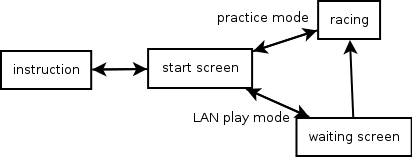
\includegraphics[scale=0.6]{state-diagram.png}
    \paragraph{}
        The start screen is displayed first, asking the player to choose a game mode to play, or to read the instruction. If practice mode is chosen, the game start directly. Otherwise if LAN play is chosen, the player has to wait for other players in the waiting screen until all players get ready.
\section{Milestone plan}
\paragraph{}
    The whole project is divided into 4 stages.
    \subsection*{Stage 1:Physics Details}
    \paragraph{}
        In this stage I'll do some research about the physics related with driving and car drifting. I'll try the Pymunk\footnote{https://code.google.com/p/pymunk/} library, which simplifies physical analysis.
    \subsection*{Stage 2:Networking Details}
    \paragraph{}
        In this phrase I'll be working on the connecting problem. I should choose a good strategy for connecting, e.g. UDP or TCP connection. Also how data is organized and transferred should be considered, too. Maybe I should synchronize all player before every frame update. Another problem is that how players can find each other so that a match can be organized quickly(maybe through UDP broadcast?).
    \paragraph{}
        I'll find a suitable library to do the work.
    \subsection*{Stage 3:Building the working game}
    \paragraph{}
        With the progress gained in stage 1 and 2, I should be able to build the working game. Graphical stuff will be done with GIMP or mtpaint. I'll work on the music later using Hydrogen, Rosegarden, Jack, Ardour, etc.
    \subsection*{Stage 4:Improvement}
    \paragraph{}
        I want to do these two improvements if time permits,
    \\
    \begin{itemize}
        \item Refine the graphical and musical design
        \item Make the game playable through the internet.
        \item A match can be ``recorded'', so that the player can play with himself/herself in the practice mode.
    \end{itemize}
\section{Data plan}
    \subsection*{Track}
    \paragraph{}
        The track is stored in a bitmap-like fashion. Every pixel has its properties, for example, whether it's an obstacle, how about the fraction at this place.
    \subsection*{Synchronization}
    \paragraph{}
        The only thing that will be transferred is the commands(turn left, brake, etc.) by the players. The commands from other player controlled \emph{his/her} car on \emph{your} screen. So action should be synchronized before the update of every frame. And the game should promise that the same series of commands will always produce the same outcome.
    \subsection*{Record}
        If time permits I'll try to implentment recording the game. Since the same series of commands will always produce the same result, the only thing that need record is the commands.
\end{document}
